% % % % % % % % % % % % % % % % % % % % % % % % % % % % % % % % % % % % % % % % %
% INTRO
% % % % % % % % % % % % % % % % % % % % % % % % % % % % % % % % % % % % % % % % %
\section{Time box 6}
\listoftodos
\subsection{Time box planning}

\begin{figure}[H]
	\begin{centering}
		\missingfigure{Updated timebox figure}
		%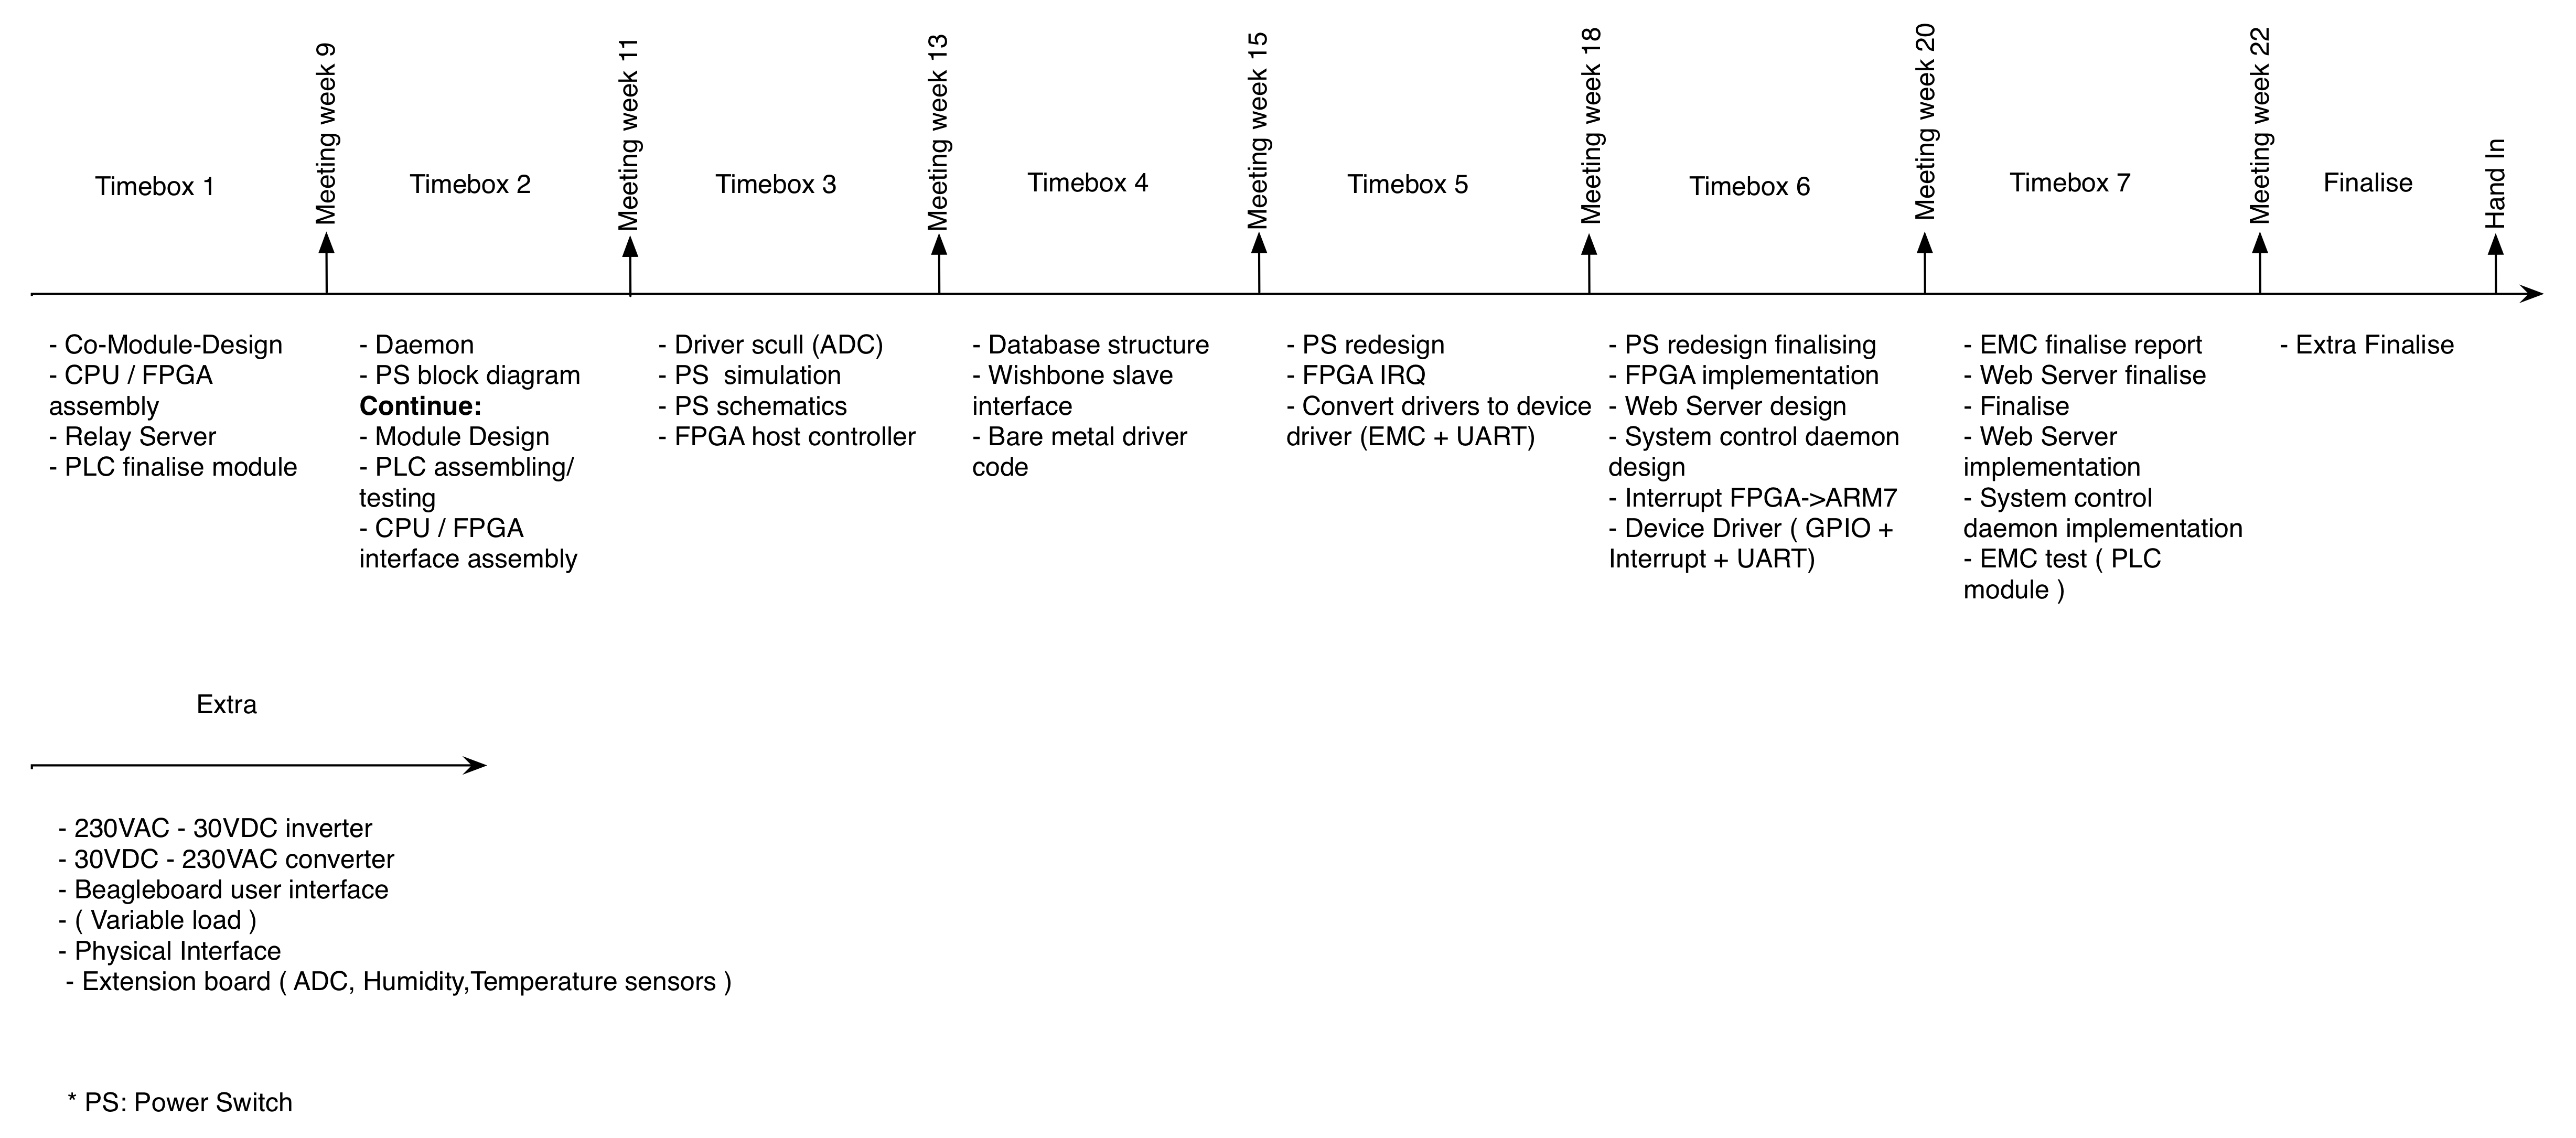
\includegraphics[width=1.0\textwidth]{images/tb_r5.png}
		%\caption{Updated time-box}
	\end{centering}
\end{figure}

\subsubsection{Work to be done in this time box}
\todo[inline]{Update List}
\begin{itemize}
	\item Theis thing
	\begin{itemize}
		\item Sub thing
	\end{itemize}
	\item Jesus thing
		\begin{itemize}
			\item sub thing
		\end{itemize}
	\item Dennis thing
	\begin{itemize}
		\item Sub thing
	\end{itemize}
\end{itemize}

\paragraph{Description:}
\todo[inline]{Update Description}
\begin{description}
	\item[Theis thing]
	\item Web Server - 
	\item[Dennis thing]
\end{description}

\subsubsection{Time planning}

\begin{table}[H]
\centering
	\todo[inline]{Update Time}
	\begin{tabular}{|l|c|c|c|c|c|}
		\hline
		~			& Theis thing			& WebServer		& Dennis thing	\\ \hline
		Estimation	& xx					& xx				& xx			\\
		Actual		& xx					& xx				& xx			\\
		Developer	& Theis					& Paulo				& Dennis		\\
		\hline
	\end{tabular}
	\caption{Estimation and actual time used on the project}
\end{table}
% % % % % % % % % % % % % % % % % % % % % % % % % % % % % % % % % % % % % % % % %
% % % % % % % % % % % % % % % % % % % % % % % % % % % % % % % % % % % % % % % % %
% Theis Thing
% % % % % % % % % % % % % % % % % % % % % % % % % % % % % % % % % % % % % % % % %
\subsection{Theis thing - Theis}
%			Intro
%					verification specification
%					deployment specification
%
\subsubsection{Analysis}
%			Analysis
%
%                Refactored block diagram
%                Refactored class diagram
%                Detailed use cases
%                User interface specification
%                System interface specification
%                Dimensioning specification 
%
\subsubsection{Design}
%       	 Design
%
%                UML/SysML deployment view(s)
%                Mechanical specifications and dimensioning
%                HW module specification per block
%                UML SW deployment view
%                Class specification
%                Refactored class diagram
%                Use case scenarios specifications
%                Sequence diagrams
%
\subsubsection{Implementation}
%     	   Implementation
%
%                Mechanical drawings with details explained
%                Electronic diagrams with details explained
%                Source code with details explained
%                Description of integration 
%
\subsubsection{Verification}
%       	 Verification
%
%                Module tests
%                Integration tests
%                Acceptance test
\subsubsection{Conclusion}
% % % % % % % % % % % % % % % % % % % % % % % % % % % % % % % % % % % % % % % % %
% % % % % % % % % % % % % % % % % % % % % % % % % % % % % % % % % % % % % % % % %
% Jesus Thing
% % % % % % % % % % % % % % % % % % % % % % % % % % % % % % % % % % % % % % % % %
\subsection{Web Server - Paulo}
%			Intro
%					verification specification
%					deployment specification
%
In time box 4 a web server was implemented at the ip address 10.1.18.223, this is a virtual machine assign as development environment for the uClinux distribution. The server is running Apache 2, PHP version 5.1.6 and MySQL server 5.0.95.
In this time box a web services system is developed for the communication between the Embedded device and the web server and the other way around. The web page made in Project 3 is incorporated with server side scripts (PHP) for a fully functional web interface.\\
\A user with read only permissions was created:

User: eval

Pass: ede10eval\\

For evaluation reasons a web application is developed with the name SeeIt, this is a PHP web application that allows the user to see the file structure of the server and the file content, this can be seen at http://10.1.18.223/Seeit/.\\
\\The development of the energy hub web interface can be followed at:

http://e10.ede.hih.au.dk/index.php/Web\_Server\_Structure

The database structure for this project was change to a common database to all modules, the new structure can be seen at:

http://e10.ede.hih.au.dk/index.php/Common\_Database

With the credentials above, the user is able to login into the phpMyAdmin tool in the AU-Herning network at the address: http://10.1.18.223/phpMyAdmin where the database structure is implemented.\\

\subsubsection{Analysis}
%			Analysis
%
%                Refactored block diagram
%                Refactored class diagram
%                Detailed use cases
%                User interface specification
%                System interface specification
%                Dimensioning specification 
%
For a fully functional web interface the communication have to present in both direction, since some teams need to send commands from them web page to the modules.
A file structure was created in the server, where each team have is own folder where all the needed scripts, images and layout styles can be implemented without changing the common layout and requirements approved in project 3.

In this time box the follow scripts are created:
\begin{itemize}
	\item index.php
	\item savedata.php
	\item sendcmd.php
	\item saveip.php
%	\item ajax.js
%	\item login.php
%	\item cron.php
	\item db\_connect.php
	\item db\_globals.php
\end{itemize}

\paragraph{Web interface file Structure}
The file structure is still in development, as such and for the correct version the structure is updated at the address: 

http://e10.ede.hih.au.dk/index.php/Web\_Server\_Structure
%
A short description for each script can be seen bellow:
\begin{itemize}
	\item index.php - First page of the web interface.
	\item savedata.php - Webservice that save data retrieved from the module to the database.
	\item sendcmd.php - Webservice to send commands to the desired module in the system.
	\item saveip.php - Webservice necessary to save the ip address of the energy hub, this will keep the system up and running even if a change on the network is made.
%	\item ajax.js - This Javascript handle AJAX requests when the page have no need to be reloaded, that ensure less bandwidth in the web server.
%	\item login.php  - This PHP script makes the authentication of the user, creating a session when the user gives the right certifications.
%	\item cron.php  - Cron jobs are running by the server in a predefined time, in this case the cron.php at the web server root will point to the cron jobs inside each module folder.
	\item db\_connect.php - Handle the connection to the MySQL database.
	\item db\_globals.php - Includes all the global variables with the credentials for the database.
\end{itemize}

\lineparagraph{Communication}
The server have to save the data retrieved from the system and send commands to the modules connected to the energy hub. Two main scripts are created: \textit{savedata.php} this script capture the values send by the HTTP request has a POST method saving them to the database and \textit{sendcmd.php} enables the user to send commands to a precise module in the system or even the energy hub.
\newpage
Measurements to be saved in the database:
\begin{figure}[H]
	\begin{centering}
		%\missingfigure{Communication savedata.php}
		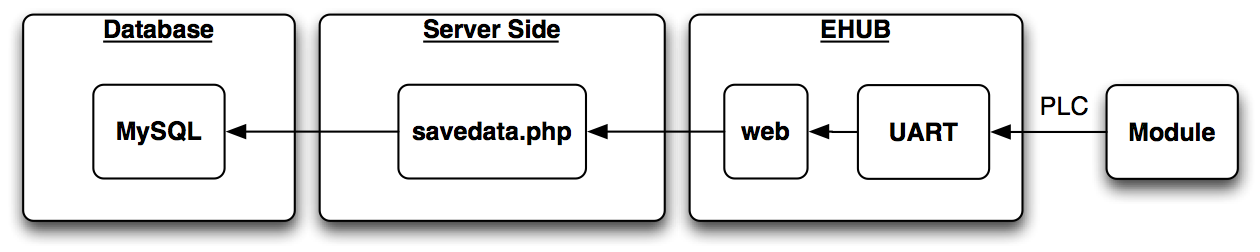
\includegraphics[width=1\textwidth]{images/tb6_webserver_savedata.png}
		\caption{Save measurements retrieved by the modules}
	\end{centering}
\end{figure}
To retrieve the measurements from the modules, an application running at the energy hub translate the data retrieved from the module through PLC to a URL request at the web server. In the server side the web server will collect the data and save it in the database.

Flow of the communication from the user until the final destination in this case the module or the energy hub.
\begin{figure}[H]
	\begin{centering}
		%\missingfigure{Communication SendCmd.php}
		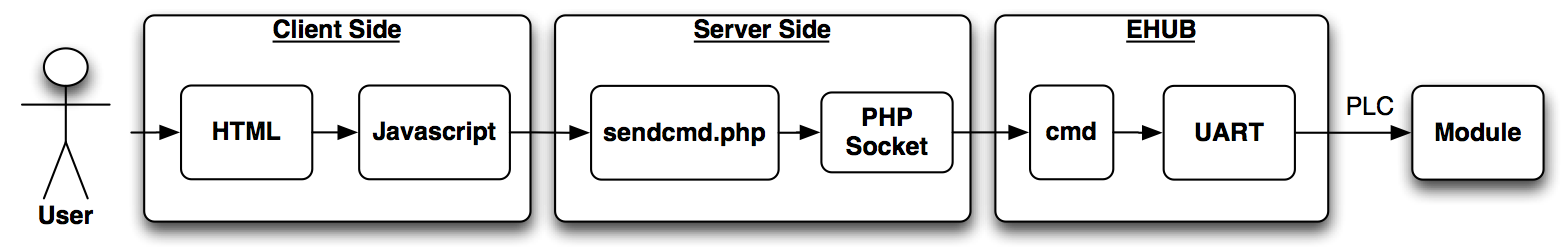
\includegraphics[width=1\textwidth]{images/tb6_webserver_sendcmd.png}
		\caption{Send a command to a module}
	\end{centering}
\end{figure}
This script doesn't give a feedback to the user, the commands send are not verified by the web server or the energy hub. The commands are handle by each module. With this system the flexibility of the system is ensured, since new modules can be added with different functionalities from the already known.
An application running in background at the energy hub OS, ensure that the command is translated to UART so it can be send through the power line communication to the modules.
\\

IP address is send from the Embedded Device:
\begin{figure}[H]
	\begin{centering}
		%\missingfigure{Communication SendCmd.php}
		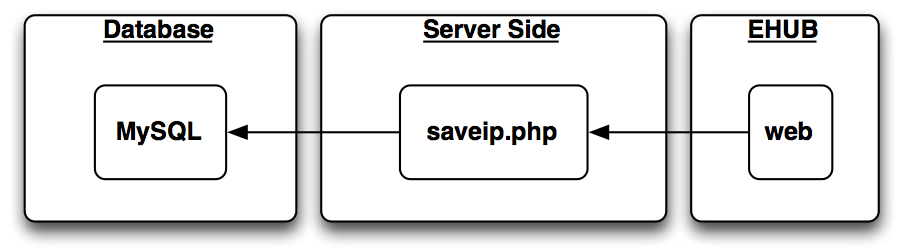
\includegraphics[width=0.8\textwidth]{images/tb6_webserver_saveip.png}
		\caption{Save the IP address of the Embedded device}
	\end{centering}
\end{figure}
A background application running (daemon), ensure that after a reboot, the IP address assigned by DHCP to the energy hub is saved in the database so commands can be send through the web interface. This add flexibility to the system, since a change in the internal network could stop the normal work of the system.

\lineparagraph{Structure Generals}

A folder is created for each team, it will contain the necessary scripts to show data for the users, send commands to the energy hub, make their own layout, etc.

This is a necessary structure for this project, since the requirements are different for all the teams. For example the energy hub page needs to show completely different data from the wind turbine or other modules.

In real production software a general layout and data should be set for all the modules pages, being possible to make small adjustments to satisfy the final user/client. This way the final software would have a improved user experience since the layout is equal in all the modules.

\subsubsection{Design}
%       	 Design
%
%                UML/SysML deployment view(s)
%                Mechanical specifications and dimensioning
%                HW module specification per block
%                UML SW deployment view
%                Class specification
%                Refactored class diagram
%                Use case scenarios specifications
%                Sequence diagrams
The main structure for the correct work of the system is created, in the next time box the energy hub page is built to allow the user to stop and start modules, get the current efficiency as green energy system, etc.

\subsubsection{Implementation}
%     	   Implementation
%
%                Mechanical drawings with details explained
%                Electronic diagrams with details explained
%                Source code with details explained
%                Description of integration 
%
\lineparagraph{index.php}

The \textit{index.php} is the main page of the system, this will redirect the users to the modules or login page.
The efficiency of the system can be seen on the first page as the amount of lamps able to power, the money saved and the mount of less CO2 emissions, this is not available in this version, will be part of the hub web page development in next time box.

\lineparagraph{savedata.php}

A background application running in the energy hub converts the measurement sent through PLC (UART) to a HTTP request \textbf{savedata.php?sensor\_id=ID Sensor\&value=Sensor Measurement\&hub\_port=Hub Port}.

\begin{lstlisting}[language=php]
<?php
	
	require_once("db_connect.php");
	
	$date = getdate();
	
	$today = $date['year'].'-'.$date['mon'].'-'.$date['mday'].' '.$date['hours'].':'.$date['minutes'].':'.$date['seconds'];

	if(isset($_GET['sensor_id']) && isset($_GET['value']) && isset($_GET['hub_port'])){
		$sql= "INSERT INTO `iEnergy`.`MEASUREMENTS` (".
			  "`ID_MEASURE` ,".
			  "`ID_SENSOR` ,".
			  "`DATE_TIME` ,".
			  "`HUB_PORT` ,".
			  "`VALUE`)".
			  "VALUES (NULL , '".$_GET['sensor_id']."', '".$today."', '".$_GET['hub_port']."', '".$_GET['value']."')";
	
		$con->query($sql); // Run the query in the MySQL server
		
		// No feedback needed since the energy hub will not expect an answer.
		
	} else {
		echo 'Incorrect parameters';
	}
	
?>
\end{lstlisting}

This script saves the measurement retrieved from a sensor to the database. At first it established the connection to the MySQL server so SQL requests can be made.
A PHP function returns an array with the current date and time, this is formatted into YYYY-M-D H:M:S, after it can be saved to the MEASUREMENTS table. The script collects all the parameters send through the URL encoding GET, a SQL code is generated and a request made to the MySQL server, the data is added to the MEASUREMENTS table.

\lineparagraph{sendcmd.php}

The web interface is able to send commands to the energy hub and the modules using the\\ \textbf{sendcmd.php?id\_module=\textless module id\textgreater\&cmd=\textless command to be send\textgreater }. The id\_module tells the hub which module the command should be send.
No verification is made of the send command by the web server or the energy hub unless the command is specifically send to the hub.

\begin{lstlisting}[language=php]

	// SQL request for the device page.
	require_once("includes/db_connect.php");
	
	if(isset($_GET['cmd']) && isset($_GET['id_module'])){
	
		$device_port = 5555;
		
		//echo 'Module Id: '.$_GET['id_module']."<BR>Command: ".$_GET['cmd']."<BR>";
		
		$sql= "SELECT IP ". 
			  "FROM `DEVICE` ". 
			  "ORDER BY ID_DEVICE DESC ".
			  "LIMIT 1";
		
		$res = $con->query($sql); // Run the query in the MySQL server
		
		$row = $res->fetch_row();
		
		$device_ip = $row[0];
		
		if ($socket=socket_create(AF_INET, SOCK_STREAM, SOL_TCP)){
			echo "Socket created <br>";
		}
	
		if (socket_connect($socket,$device_ip,$device_port)){
			echo "Connection stablished<br>";	
		} else {
			exit (socket_strerror(socket_last_error()));
		}
	
		$str = $_GET['cmd'].';'.$_GET['id_module'];
		
		socket_write($socket,$str);
	
		socket_close($socket);
		
	} else {
		echo 'Command or Module Id not set';
	}
\end{lstlisting}

At first the script will get the ip address of the energy hub, running a SQL code that retrieves the last IP address added to the table DEVICE. With the energy hub ip and a predefined port, a connection is created using a TCP socket for the communication. The command and the module id are send and the socket is closed.

\lineparagraph{saveip.php}

\textit{saveip.php} script is called by the background application running on the embedded device, it saves the IP address given by DHCP, this is used for further communication between the web server and the energy hub.
\begin{lstlisting}[language=php]
	require_once("includes/db_connect.php");

	if(isset($_GET['ip'])){
		$sql= "INSERT INTO `iEnergy`.`DEVICE` (".
			  "`ID_DEVICE` ,".
		  	  "`IP`)".
		  	  "VALUES (NULL , '".$_GET['ip']."')";
	
		$con->query($sql); // Run the query in the MySQL server
		
		// No feedback needed since the energy hub will not expect an answer.
		
	} else {
		echo 'IP not set';
	}
\end{lstlisting}
The ip address is send by the GET method (saveip.php?ip=127.0.0.1), this is how the data in encoded into a URL, being collected in the variable \$\_GET['ip']. 
A \$sql variable string is created containing the SQL code to be run at the MySQL server.

\lineparagraph{db\_connect.php}

For the communication to the database a driver is used in PHP that provides an interface to the MySQL server. The PHP mysqli extension (MySQL improved) is used in this project, this is recommend for MySQL servers version 4.1.3 or later. This extension provides several benefits as a objective-oriented interface, support for multiple statements, embedded server support and more can be found in the MySQL documentation.

\begin{lstlisting}[language=php]
	require_once("db_globals.php");
	
	$con = new mysqli(DB_HOST,DB_USER,DB_PASS,DB_NAME); // Creates new mysql connection
	
	if($con->connect_error){
		echo "Failed to connect to MySQL: (" . $con->connect_errno . " ) ". $con->connect_error;
	} 
	else { echo "Connection established"; }
\end{lstlisting}

In this script an object is instantiated with a connection to the MySQL server.

\textit{\$con = new mysqli\textless parameters \textgreater)}

The parameters are included from the db\_globals.php, setting the server host, user, password and database to be used.

\lineparagraph{db\_globals.php}

Using a script to define the parameters for the MySQL connection, 
All the scripts that need to use the global parameters for the connection to the MySQL server, should include db\_globals.php as shown in the db\_connect.php above.

\begin{lstlisting}[language=php]
	// MySQL condifuration
	DEFINE ('DB_USER','root');
	DEFINE ('DB_PASS','root');
	DEFINE ('DB_HOST','localhost');
	DEFINE ('DB_NAME','iEnergy');
\end{lstlisting}

The global parameters the connection to the MySQL server are define in this script.

\begin{itemize}
	\item DB\_USER - Database user name with read, write and execute permissions.
	\item DB\_PASS - Password for the user
	\item DB\_HOST - Hostname for the MySQL server, if running at the same host as the PHP server, localhost or 127.0.0.1 should be used.
	\item DB\_NAME - Database name to connect to.
\end{itemize}

\subsubsection{Verification}
%       	 Verification
%
%                Module tests
%                Integration tests
%                Acceptance test
The verification is made using the tools described in the beginning of this section:
\begin{table}[H]
\centering
	\begin{tabular}{| c | l | c |}
		\hline
		Verification & Description & Acceptance \\\hline
		1 & Save new IP address: saveip.php?ip=127.0.0.1 & OK \\\hline
		2 & Send command: sendcmd.php?unique\_id=0\&cmd=led 1 on & TimeBox7 \\\hline
		3 & File structure created & OK \\\hline
	\end{tabular}
\end{table}

\subsubsection{Conclusion}
The common web services and file structure in the web server was created for all the modules/teams.\\
The implementation of the savedata.php will required further analysis for a working system, since the energy hub needs to have a table of all the sensors connected to each module. When a module retrieves a value the hub needs to know which sensor the measurement belongs to. This was not taken in consideration in earlier analysis of the system and might affect the protocol developed and system dynamics.\\
In the next time box a scaled down prototype is developed and the communication dynamics between web server and modules can be tested.

% % % % % % % % % % % % % % % % % % % % % % % % % % % % % % % % % % % % % % % % %
% % % % % % % % % % % % % % % % % % % % % % % % % % % % % % % % % % % % % % % % %
% Dennis Thing
% % % % % % % % % % % % % % % % % % % % % % % % % % % % % % % % % % % % % % % % %
\subsection{Dennis thing - Dennis}
%			Intro
%					verification specification
%					deployment specification
%
\subsubsection{Analysis}
%			Analysis
%
%                Refactored block diagram
%                Refactored class diagram
%                Detailed use cases
%                User interface specification
%                System interface specification
%                Dimensioning specification 
%
\subsubsection{Design}
%       	 Design
%
%                UML/SysML deployment view(s)
%                Mechanical specifications and dimensioning
%                HW module specification per block
%                UML SW deployment view
%                Class specification
%                Refactored class diagram
%                Use case scenarios specifications
%                Sequence diagrams
%
\subsubsection{Implementation}
%     	   Implementation
%
%                Mechanical drawings with details explained
%                Electronic diagrams with details explained
%                Source code with details explained
%                Description of integration 
%
\subsubsection{Verification}
%       	 Verification
%
%                Module tests
%                Integration tests
%                Acceptance test
\subsubsection{Conclusion}
% % % % % % % % % % % % % % % % % % % % % % % % % % % % % % % % % % % % % % % % %
% % % % % % % % % % % % % % % % % % % % % % % % % % % % % % % % % % % % % % % % %
% Deployment
% % % % % % % % % % % % % % % % % % % % % % % % % % % % % % % % % % % % % % % % %
\subsection{Deployment}
	%which versions of the prototype the customer will get
	%with what functionality.
\paragraph{Theis thing}
%
%
\paragraph{Jesus thing}
%
%
\paragraph{Dennis thing}
%
%